\section{El desafortunado profesor Santa María}

El profesor Santa María ha sufrido un accidente y para salvar su vida es necesario realizarle una transfusión sanguínea. El problema es que el profesor Santa María es grupo B RH-, el cual es sumamente escaso. Para buscar posibles donantes, el profesor Santa María ha realizado un código en Python que genera un archivo (\texttt{sangre.txt}) a partir de dos bases de datos de la Universidad (\texttt{alumnos\_1.txt} y \texttt{alumnos\_2.txt}).
\begin{figure}[h]
    \centering
    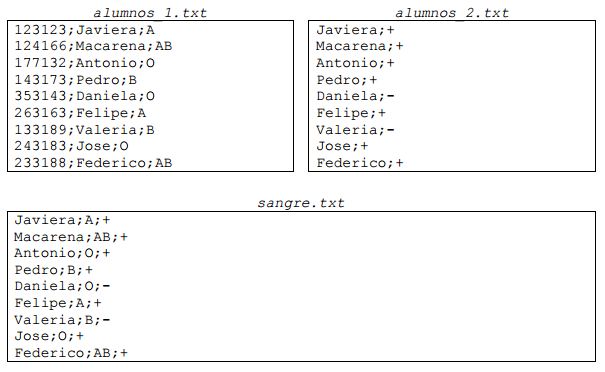
\includegraphics{Imagenes/sangre.png}
\end{figure}

Como el profesor Santa María está gravemente herido, el código se desordenó al guardarlo, por lo que le pide a usted que ordene las líneas de código coherentemente considerando indentaciones y sintaxis del lenguaje.

\begin{figure}[h]
    \centering
    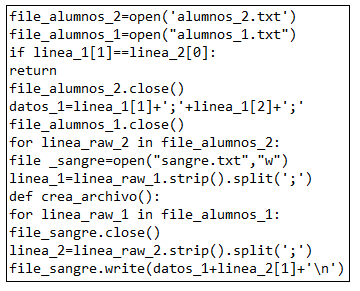
\includegraphics[scale=0.9]{Imagenes/desorden.png}
\end{figure}

\paragraph{Desafío} El profesor Santa María ha entrado en estado crítico y ya no es capaz de escribir funciones en Python por sí mismo. De usted depende salvar la vida de este estimado docente.
Considere el archivo \texttt{compatibilidad.txt} que ha sido previamente generado a partir de la matriz receptor/donante

\begin{figure}[h]
    \centering
    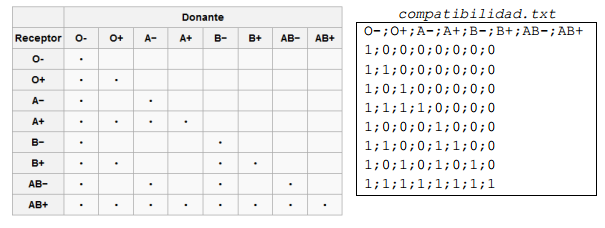
\includegraphics{Imagenes/compatibilidad.png}
\end{figure}

Considere también el archivo \texttt{sangre.txt}. Además, conociendo al profesor Santa María, tenga en cuenta que el no escribiría funciones que sirvieran únicamente a su propósito, sino que se esforzaría en crear funciones genéricas que sirvieran para cualquier tipo de sangre.


Escriba la función \texttt{donantes(tipo\_sangre)} que genere un archivo llamado \texttt{donantes.txt} a partir del archivo \texttt{sangre.txt} y del archivo \texttt{compatibilidad.txt}. El archivo creado debe contener únicamente la información de aquellos alumnos que resulten ser donantes compatibles para \texttt{tipo\_sangre}.

\begin{lstlisting}[style=consola]
>>> [*donantes('B-')*]
>>> [*arch=open('donantes.txt')*]
>>> [*for linea in arch:*]
        [*print linea.strip()*]

Daniela;O;-
Valeria;B;-

>>> [*arch.close()*]

\end{lstlisting}